\chapter{Моделирование систем из нескольких РЛС}

\section{Теоретическая часть}

Объединение двух РЛС с идентичными параметрами $D$ и $F$ позволяет получить схемы объединения РЛС по различным критериям, означающими принятие решения в пользу альтернативы при данном решении для определенного количества РЛС. Данный принцип порождает две минимаксные схемы «И» и «ИЛИ». Объединение по схеме «ИЛИ» приводит к улучшению $D(D_c > D)$, но ухудшает $F(F_c > F)$, и наоборот, схема «И» ухудшает $D(D_c < D)$, но улучшает $F(F_c < F)$. В схеме объединения «И» вероятности будут определяться как $F_1 = F_2 = \sqrt{F_c} = \sqrt{F_e}$ где $F_c$ – вероятность ЛТ эквивалентной РЛС, а $F_e$ – вероятность ЛТ комплекса.
В схеме «ИЛИ» эти вероятности будут равны $F_1 = F_2 = 1 - \sqrt{1 - F_c} = 1 - \sqrt{1 - F_e}.$
В данной работе рассматривается ситуация объединения 4 и 18 РЛС. 

\section{Моделирование системы из 4 РЛС}

\begin{figure}
    \centering
    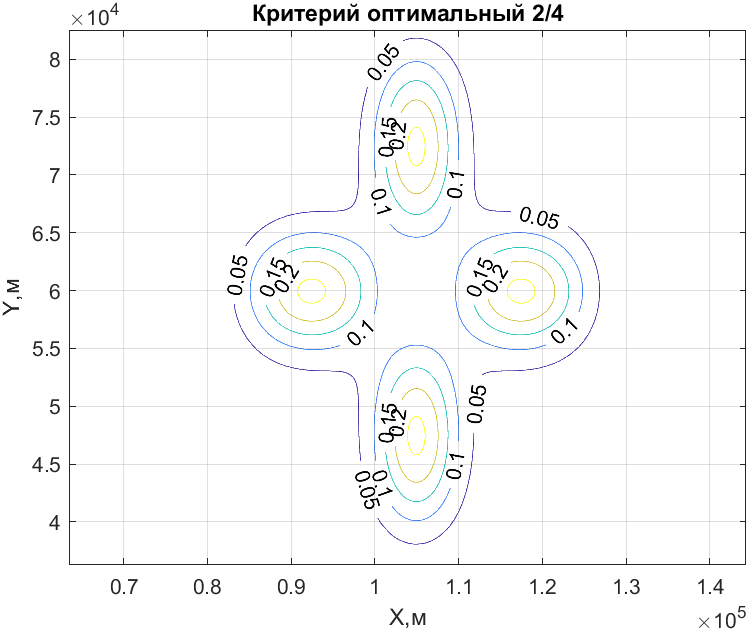
\includegraphics{figures/2_4_RLS.png}
    \caption{Критерий 2 из 4 для 4х РЛС}
    \label{fig:my_label}
\end{figure}

\begin{figure}
    \centering
    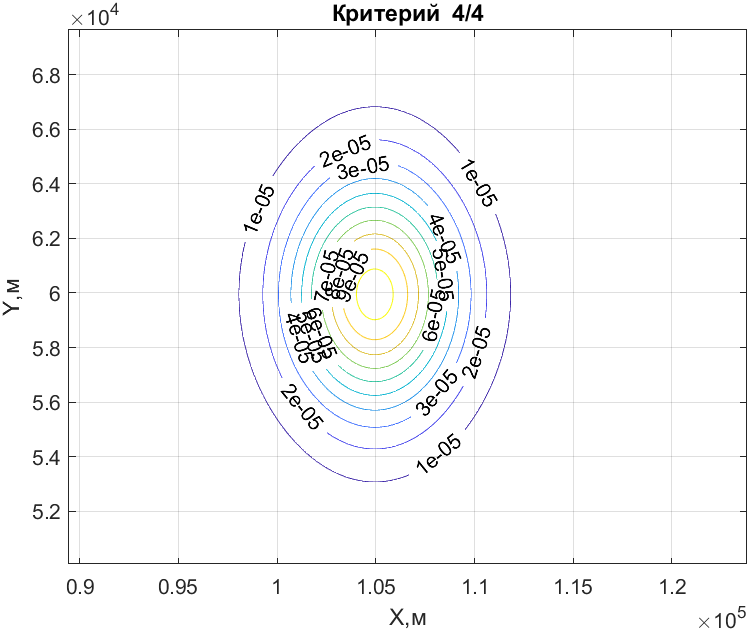
\includegraphics{figures/4_4_RLS.png}
    \caption{Критерий 4 из 4 для 4х РЛС}
    \label{fig:my_label}
\end{figure}

\begin{figure}
    \centering
    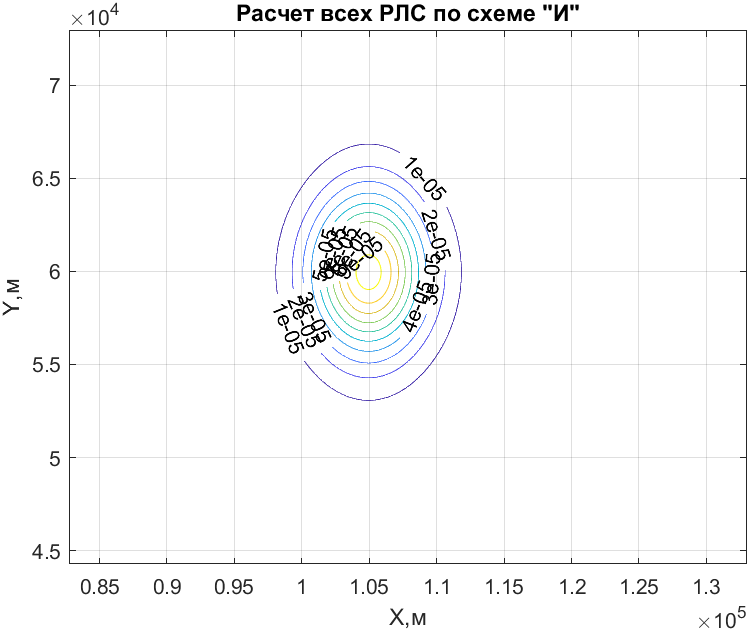
\includegraphics{figures/AND_RLS_4.png}
    \caption{Объединение для 4х РЛС по схеме "И"}
    \label{fig:my_label}
\end{figure}

\begin{figure}
    \centering
    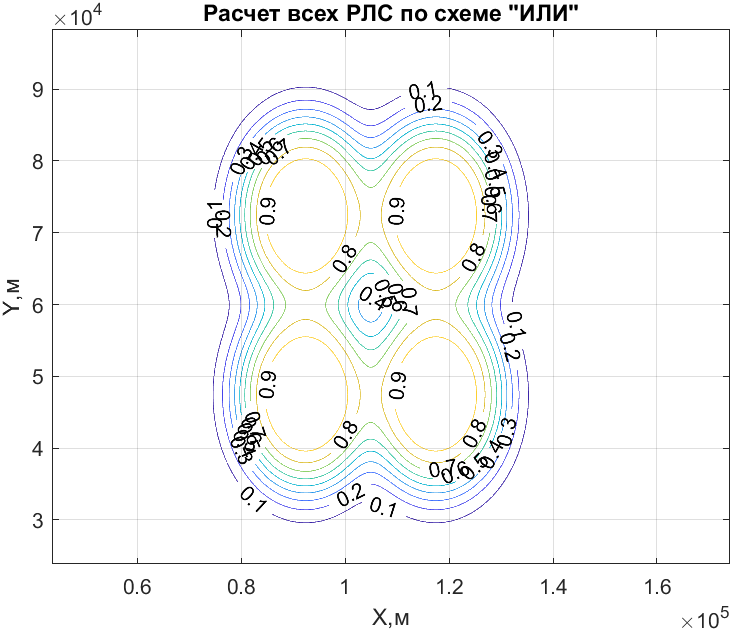
\includegraphics{figures/OR_RLS_4.png}
    \caption{Объединение для 4х РЛС по схеме "ИЛИ"}
    \label{fig:my_label}
\end{figure}

\begin{figure}
    \centering
    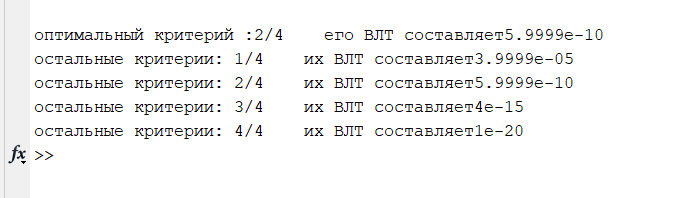
\includegraphics[scale = 0.7]{figures/VLT_4.png}
    \caption{Вероятность ложной тревоги для 4 РЛС}
    \label{fig:my_label}
\end{figure}

\section{Моделирование системы из 18 РЛС}

\begin{figure}
    \centering
    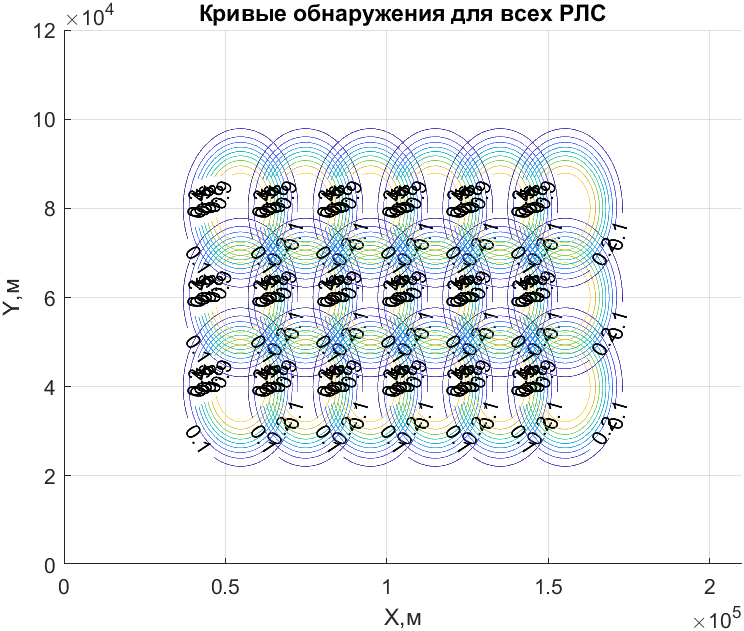
\includegraphics{figures/ALL_RLS.png}
    \caption{Кривые обнаружения для всех РЛС}
    \label{fig:my_label}
\end{figure}

\begin{figure}
    \centering
    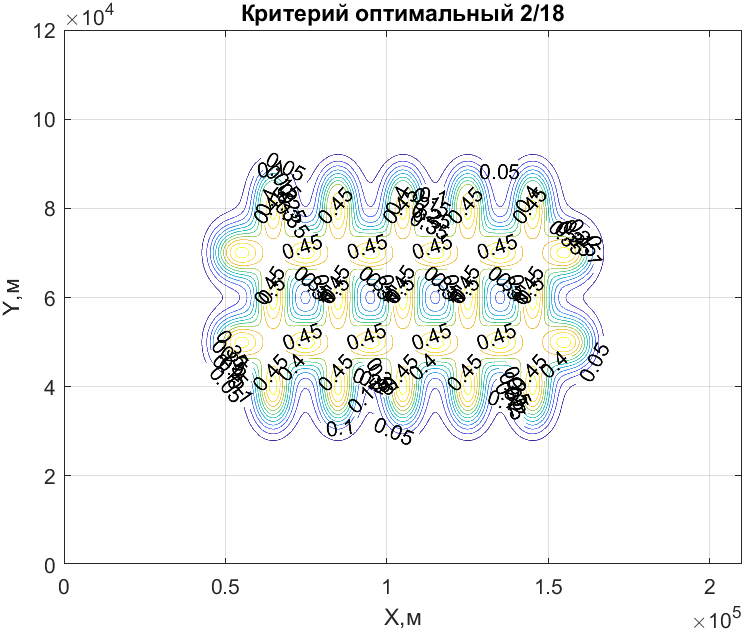
\includegraphics{figures/2_18_RLS.png}
    \caption{Оптимальный критерий обнаружения для 18 РЛС}
    \label{fig:my_label}
\end{figure}

\begin{figure}
    \centering
    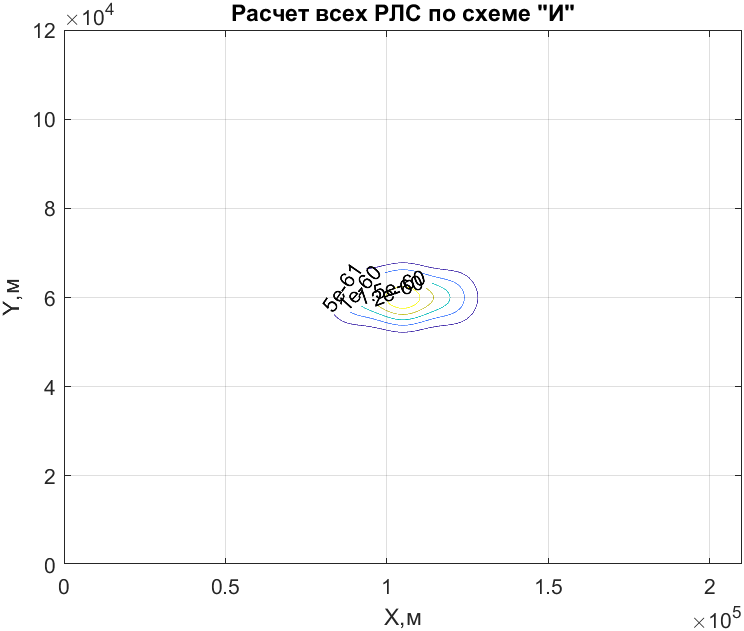
\includegraphics{figures/AND_RLS_18.png}
    \caption{Объединение всех РЛС по схеме "И"}
    \label{fig:my_label}
\end{figure}

\begin{figure}
    \centering
    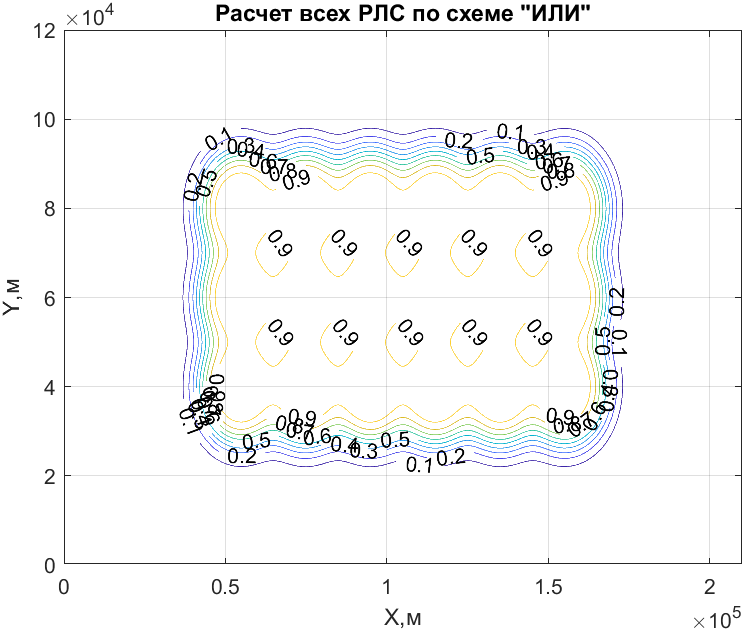
\includegraphics{figures/OR_RLS_18.png}
    \caption{Объединение всех РЛС по схеме "ИЛИ"}
    \label{fig:my_label}
\end{figure}

\begin{figure}
    \centering
    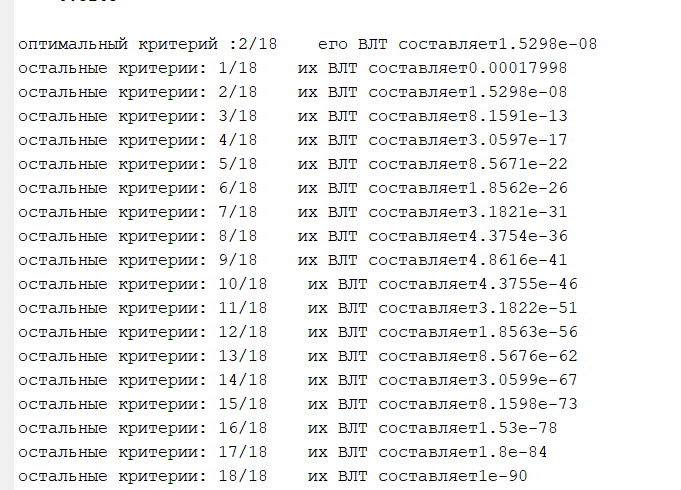
\includegraphics[scale = 0.7]{figures/VLT_18.png}
    \caption{Вероятность ложной тревоги для 18 РЛС}
    \label{fig:my_label}
\end{figure}
